
\section{Estudo dos dados}

Os dados que proponho a prever são os de Energia Usada na Banda de Reserva Secundária, tanto a subir como a descer: "UpwardUsedSecondaryReserveEnergy","DownwardUsedSecondaryReserveEnergy".\\



\begin{figure}[H]
  \centering
  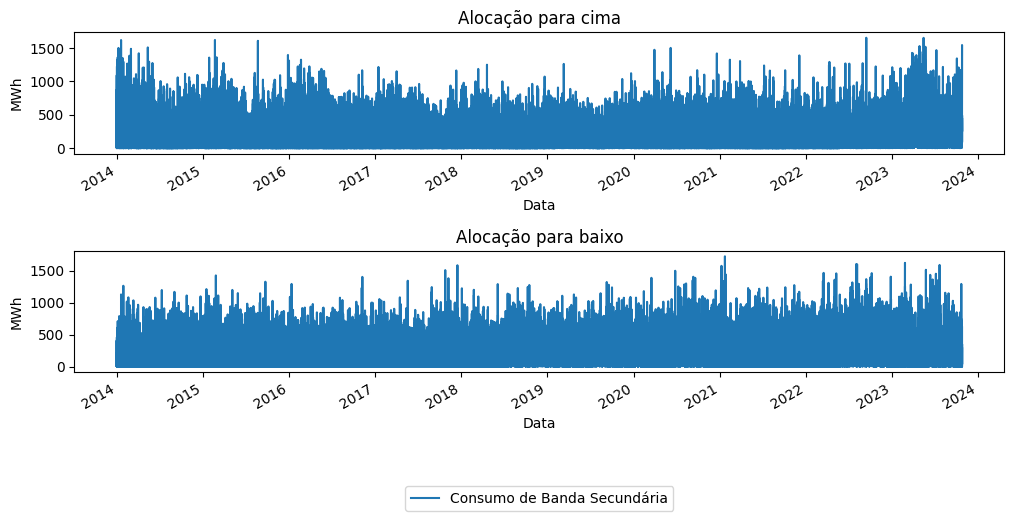
\includegraphics[width=\textwidth]{plots/consumo_originais.png}
  \caption{Serie Temporal dos dados alvo}
  \label{fig:targettimeseries}
\end{figure}


Para termos uma melhor percepção dos mesmos segue algumas janelas temporais mais pequenas.

\begin{figure}[H]
  \centering
  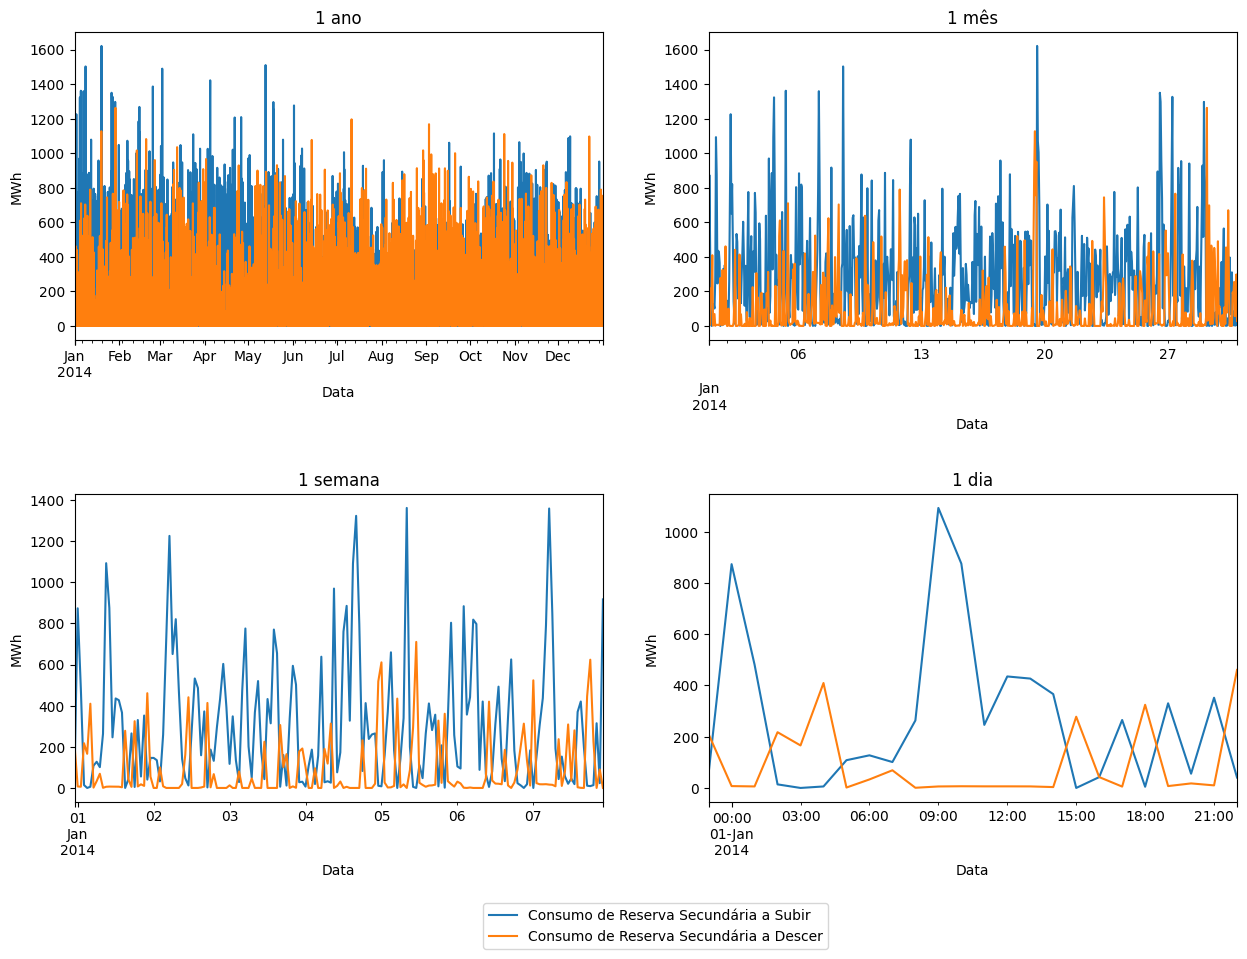
\includegraphics[width=\textwidth]{plots/target_timeseries_windows.png}
  \caption{Janelas Temporais dos dados alvo}
  \label{fig:targettimeserieswindows}
\end{figure}


Estas mostram claramente que ambos os atributos mantêm um comportamento tanto discreto, como linear, isto é, que ou existe algum valor, ou é zero, e se existe valor este tem comportamento linear.\\
A distribuição destes dados é claramente exponencial. O que é importante para a escolha de alguns parâmetros na modelação. \\

		
\begin{figure}[H]
  \centering
  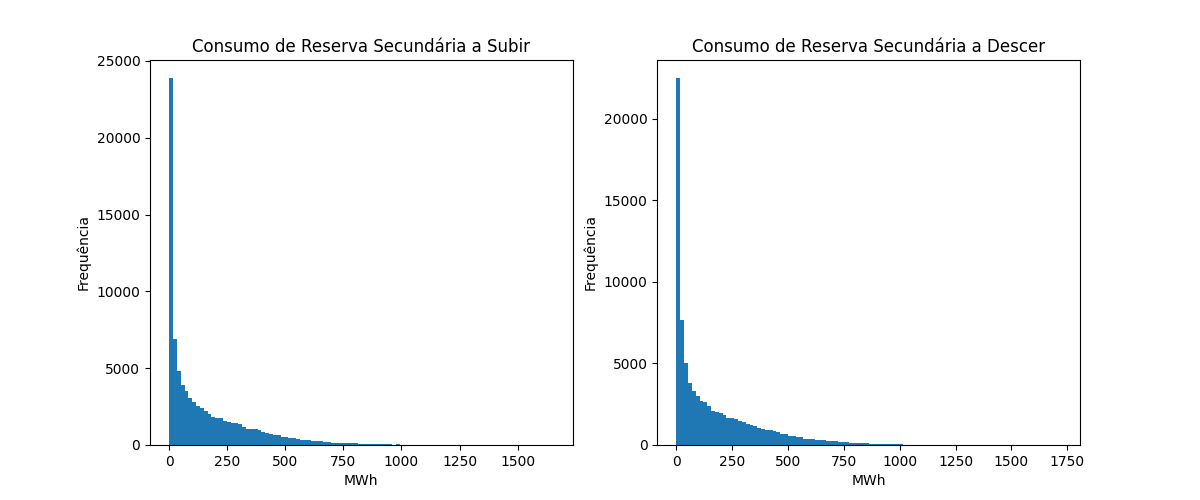
\includegraphics[width=\textwidth]{plots/target_histograms.png}
  \caption{Frequência dos dados alvos}
  \label{fig:targethistograms}
\end{figure}


\subsection{Correlações}

Os modelos vão depender bastante de correlação entre variáveis.

Nesta secção queremos tentar identificar se há visiveis relações entre as variáveis, e se há relações temporais  visiveis nas colunas alvo.


\subsubsection{Correlações entre atributos}


\begin{figure}[H]
  \centering
  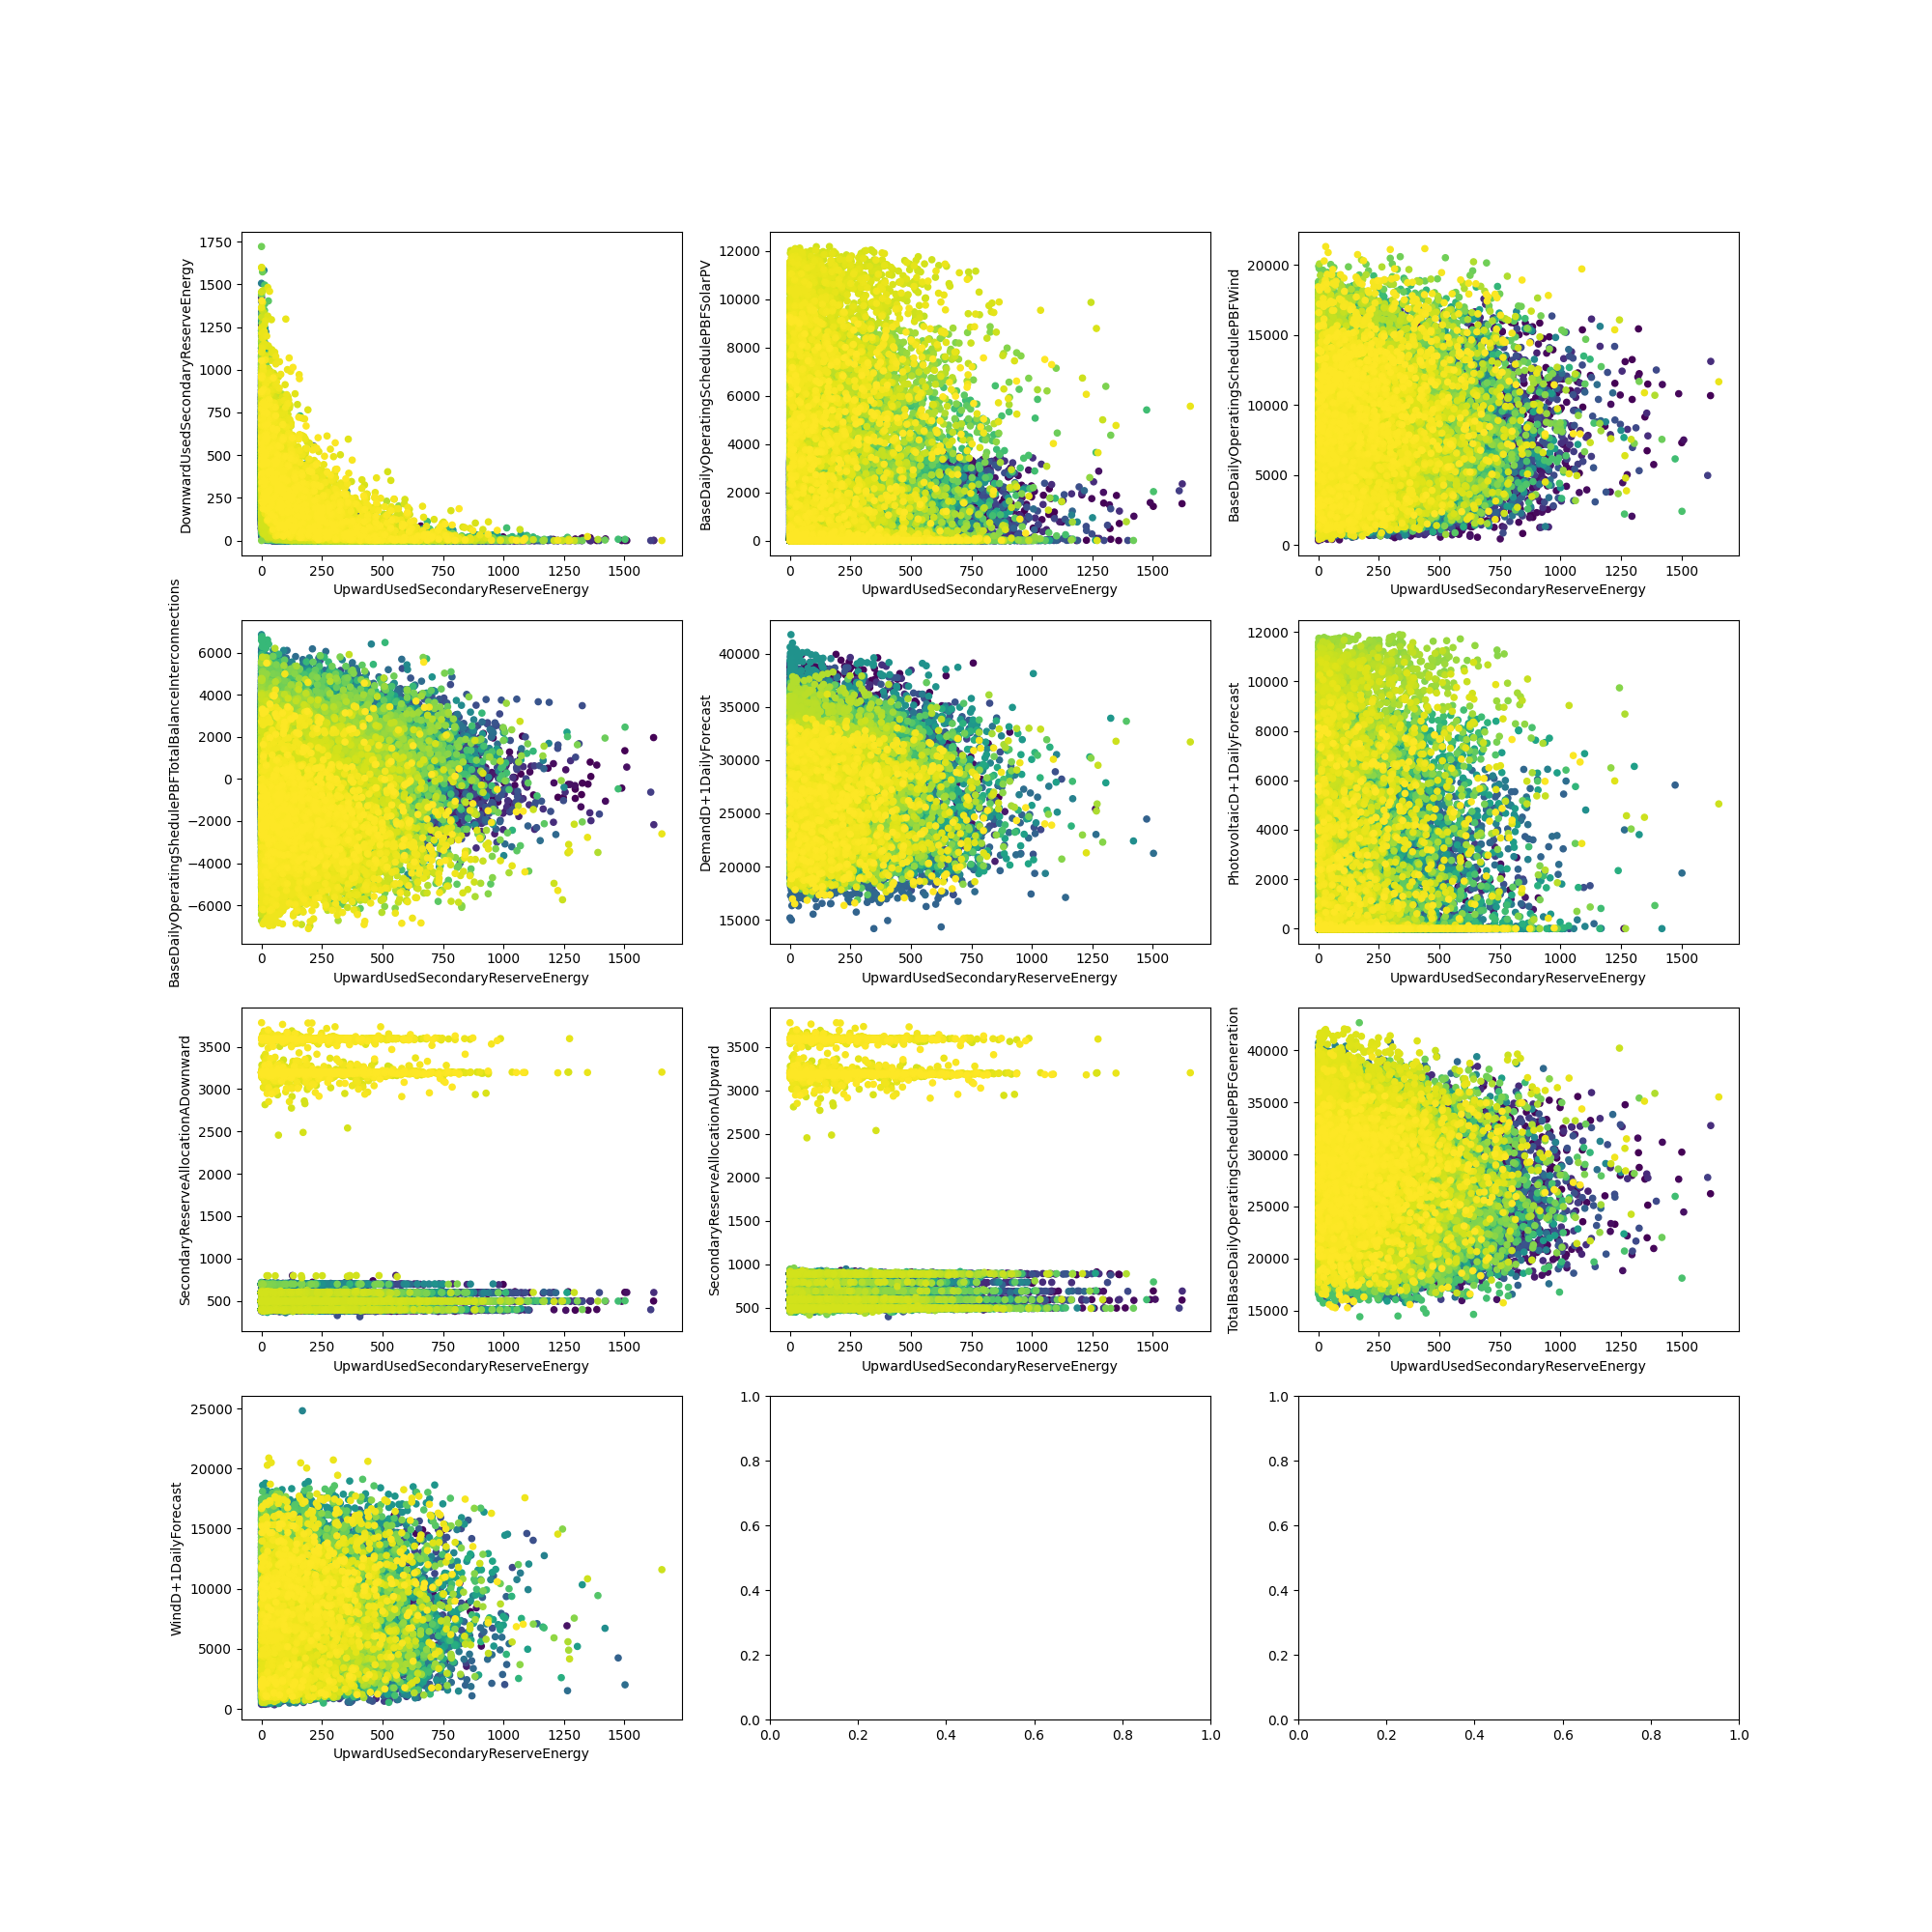
\includegraphics[width=\textwidth]{plots/feature_correlation.png}
  \caption{Correlação entre atributos}
  \label{fig:featurecorrelation}
\end{figure}

Esta figura apresenta a dispersão de valores entre a energia usada, primeiras três linhas a energia para cima e as seguintes a energia para baixo, e os outros atributos presentes.\\
As correlações entre variáveis parecem muitos escassas, o que apresenta já que a previsão destes dados usando estas variáveis vai ser um problema difícil.\\
Por norma é feito uma seleção de atributos baseado nestas correlações, eliminando assim os atributos que ajudam menos, ou até prejudicam os modelos.\\
Segue os valores de correlação onde podemos ver numericamente que existe muito pouca correlação entre os atributos. Onde a primeira coluna são os valores de correlação para a energia usada a subir e a segunda coluna as correlações da energia usada a descer.\\

\begin{figure}[H]
  \centering
  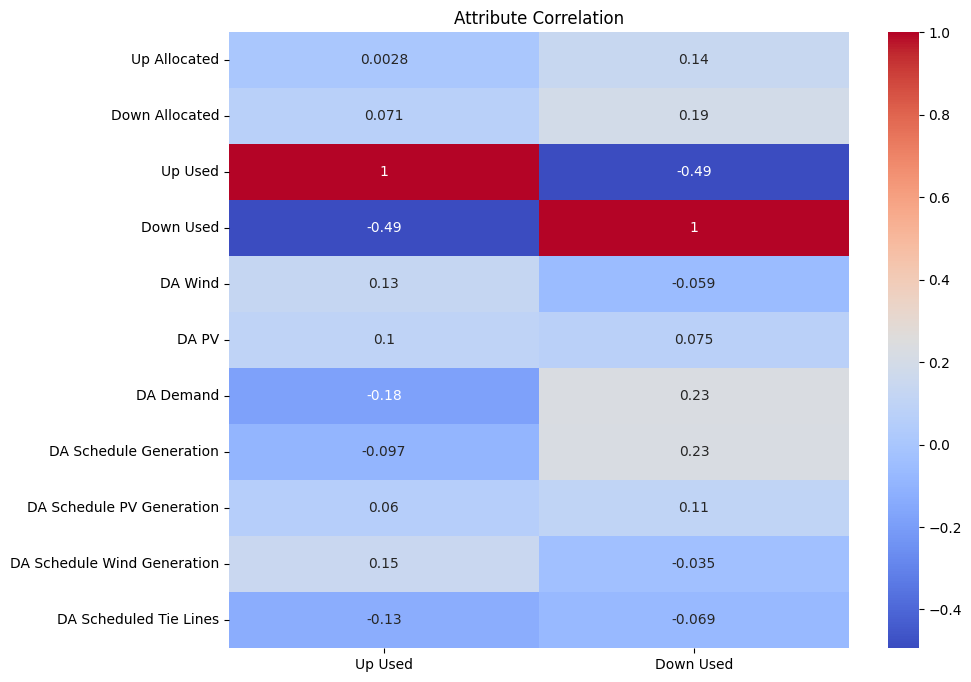
\includegraphics[width=\textwidth]{plots/correlation_heatmap.png}
  \caption{Valores de correlação entre atributos}
  \label{fig:correlationheatmap}
\end{figure}

\subsubsection{Correlações Temporais}

\begin{figure}[H]
  \centering
  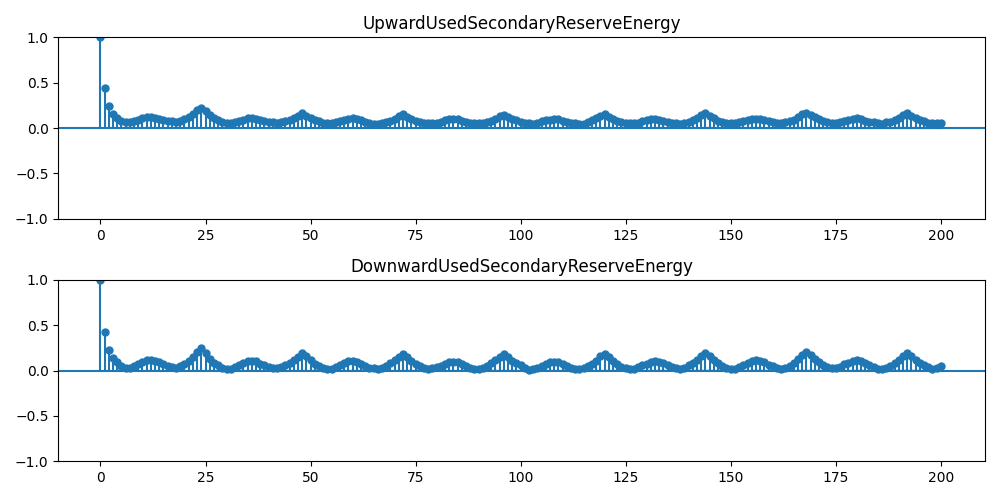
\includegraphics[width=\textwidth]{plots/autocorrelation.png}
  \caption{Autocorrelação Temporal}
  \label{fig:autocorrelation}
\end{figure}

A autocorrelação, em ambos os alvos, é mais forte nas 3 horas mais próximas, e nos pontos com diferença de 12 e 24 horas. \\
É de notar que estes valores são baixos, prometendo já também uma baixa regressividade temporal. \\
Os melhores saltos temporais e suas correlações são mostradas na tabelas em baixo:\\


\begin{table}[H]
  \caption{Autocorrelação Temporal}    
  \resizebox{\linewidth}{!}{\begin{tabular}{lllllllllll}
\toprule
\midrule
\multirow[t]{2}{*}{UpwardUsedSecondaryReserveEnergy} & horas & 1 & 2 & 24 & 23 & 25 & 168 & 144 & 192 & 48 \\
 & rácio & 0.44 & 0.24 & 0.22 & 0.19 & 0.19 & 0.17 & 0.16 & 0.16 & 0.16 \\
\cline{1-11}
\multirow[t]{2}{*}{DownwardUsedSecondaryReserveEnergy} & horas & 1 & 2 & 24 & 23 & 25 & 168 & 144 & 192 & 48 \\
 & rácio & 0.43 & 0.22 & 0.25 & 0.20 & 0.19 & 0.21 & 0.19 & 0.20 & 0.19 \\
\cline{1-11}
\bottomrule
\end{tabular}
}
  \label{tab:tempcorr}
  \end{table}

Outro ponto a denotar é que os objectos não têm um comportamento completamente linear, i.e., parece existir um comportamento discreto na questão ser alocado ou não esta reservas secundárias, e caso seja alocado, aí existir alguma linearidade. \\
Logo qualquer tipo de modelação terá de resolver primeiramente este problema. \\
Estas relações mostram que em termos de atributos usados vai ser um desafio complicado para qualquer tipo de modelo. \\
No âmbito desta dissertação queremos verificar a qualidade das previsões usando estes mesmo atributos, logo, não será feita seleção dos mesmos. \\
A nível da relação temporal, a maior parte dos modelos que iremos testar aplica um janela na dimensão temporal, usando todos os valores nessa janela, e aplicando os pesos nessas distâncias que mais se enquadram. Logo também não é relevante escolher apenas as distâncias temporais com maior correlação, pois os modelos vão fazer essa pesagem. \\


